\begin{infocard}{Ejemplo de serie o sucesión aritmética}
    La Figura \ref{fig:20230320164417} son dos ejemplos de sucesiones aritméticas. Observa sus diferencias comunes.

    \begin{figure}[H]
        \centering
        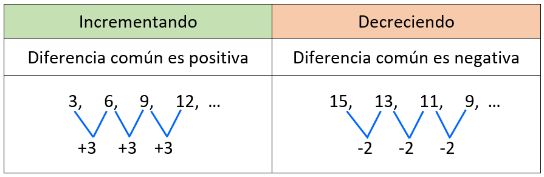
\includegraphics[width=\linewidth]{../images/20230320164417}
        \caption{Ejemplos de series aritméticas con diferencia común positiva (izquierda) y negativa (derecha).}
        \label{fig:20230320164417}
    \end{figure}
\end{infocard}